\documentclass[bars,mathserif]{beamer}

\usetheme{Dresden}
\usepackage{graphicx}
\usepackage[utf8x]{inputenc}
\usepackage{default}

\usepackage{amssymb,amsmath}
\newcommand{\bv}[1]{\mathbf{#1}} 
\newcommand{\req}[1]{#1^{*}} 
\usepackage[brazilian]{babel}

\setbeamertemplate{footline}[page number]
\setbeamercovered{invisible}
\setbeamertemplate{navigation symbols}{}
\setbeamersize{text margin left=.5cm,text margin right=.5cm} 

\title[Eulerian-Lagrangian Simulation of a Turbulent Evaporating Spray]{Eulerian-Lagrangian Simulation of a Turbulent Evaporating Spray}
\author[candidate,advisor]{Rodrigo B. Piccinini}
\institute[ITA]
{
\medskip{\emph{e-mail: rbpiccinini@gmail.com}} \\ \vspace{10pt}
  \normalsize Apresentação de Tese de Mestrado \\ \vspace{10pt}


\includegraphics[width=0.2\textwidth]{./imgs/ita_rgb.jpg} \hspace{20pt} 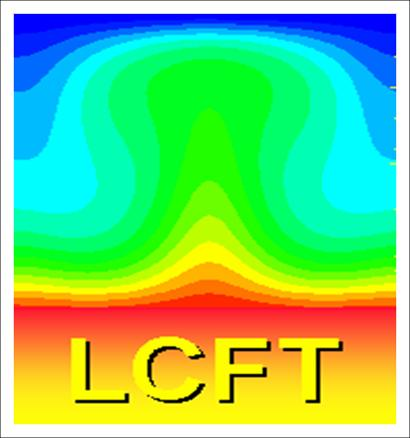
\includegraphics[width=0.1\textwidth]{./imgs/lcft.jpg} \\ \vspace{5pt}
  \footnotesize  Instituto Tecnológico de Aeronáutica \\
  Programa de Engenharia Aeronáutica e Mecânica\\
  Área de Aerodinâmica, Propulsão e Energia \\ \vspace{10pt}
\vspace{5pt}
\footnotesize Novembro, 2011.

}
\date{}
%
% Adicionar slide com o algoritmo do PISO!
%
%
\begin{document}
%
{
%   \usebackgroundtemplate{\centering\includegraphics[width=\paperwidth]{imgs/ita_cinza.png}}
  \begin{frame}[plain]
    \titlepage
  \end{frame}
} 
%
\begin{frame}
   \frametitle{Conteúdo}
   \tableofcontents
\end{frame}

\section{Introdução}
%
\begin{frame}

\begin{block}{Definição:}
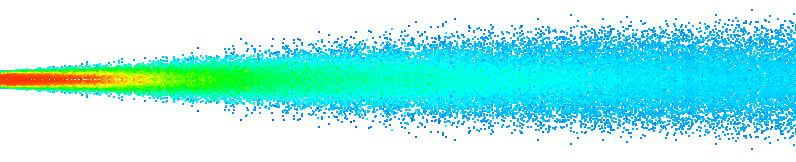
\includegraphics[width=\textwidth]{./imgs/visit/spray.png}
\end{block}

\begin{block}{Motivação:}
\begin{itemize}
 \item Aplicações em geração de energia e propulsão;
 \item Escoamento multifásico e turbulento com transferências de momento, calor e massa entre as fases.
\end{itemize}
\end{block}
\begin{block}{Tratamento das fases:}
\begin{itemize}
 \item Método Euleriano-Langragiano.
\end{itemize}
\end{block}
\end{frame}

\begin{frame}{Objetivos}
\begin{itemize}
  \item Implementar um modelo de escoamento de baixo Mach.
  \item Aplicar modelos de troca de massa, momento e energia entre as fases e um modelo de viscosidade turbulenta para descrever o jato do spray.
  \item Comparar quantidades calculadas como velocidade e diâmetro das gotas, velocidade do gás e propriedades da turbulência com experimentos relatados na literatura.
\end{itemize}
 
\end{frame}

%
\section{Equações}
\frame{\tableofcontents[currentsection]}
%
\subsection{A Fase Contínua}
%
\begin{frame}
\frametitle{Obtendo as equações da fase contínua:}
\begin{enumerate}
 \item<1-> Equações (na forma compressível) para uma mistura de gases ideais \pause + \alert{termos fontes do spray};
 \item<3-> Aproximação para baixo Mach;
 \item<5-> Escoamento médio (Reynolds e Favre);
 \item<7-> Modelo de turbulência;
\end{enumerate}
%
\begin{overprint}
\onslide<2>
\footnotesize
\centering
\begin{tabular}{|l|}
\hline
\textit{Two-way coupling} ou acoplamento em duas vias \\
\hline 
\end{tabular}

\onslide<4>
\footnotesize
\centering
\begin{tabular}{|l|}
\hline \\
Séries de potências em $\xi = \sqrt{\gamma_{\infty}} M$:\\ \\
$p = p_{0} + p_{1}\xi + p_{2}\xi^2 + O\left( \xi^3 \right)$\\
$Y_k = Y_{k,0} + O\left( \xi \right) $\\
$\bv{U} = \bv{U}_{0} + O\left( \xi \right)$ \\
$T = T_{0} + O\left( \xi \right)$ \\ \\
\hline 
\end{tabular}
%
\onslide<8>
\footnotesize
\centering
\vspace{10pt}
\begin{tabular}{|l|}
\hline
Modelo de viscosidade turbulenta (k-epsilon): \\
2 EDPs para $k$ e $\epsilon$ \\
1 Equação Algébrica para $\mu_t$ \\
Acoplamento com o spray em uma via (\textit{one-way coupling}) \\
\hline 
\end{tabular}
\end{overprint}
\end{frame}
%
\begin{frame}
\begin{block}{Equação da Continuidade:}
\begin{equation*}
  \frac{\partial \bar{\rho}}{\partial t} + \nabla \cdot \left( \bar{\rho}
\tilde{\bv{U}} \right) =  \alert{\bar{S}_m}
\end{equation*}
\end{block}
\end{frame}
%
\begin{frame}
\begin{block}{Equação das Espécies Químicas: Acetona e Ar.}
\begin{itemize}
 \pause
 \item<1-> Acetona - espécie escassa:
\begin{equation*}
 \frac{\partial \bar{\rho} \tilde{Y}_{ac} }{\partial t} + \nabla
\cdot\left(\bar{\rho} \tilde{\bv{U}} \tilde{Y}_{ac} \right) = \nabla \cdot \left[ \bar{\rho} \left( \alert{\nu + \nu_T} \right)
\nabla \tilde{Y}_{ac} \right] +\alert{\bar{S}_{Yac}}
\end{equation*}
\pause
\item<4-> Ar - espécie diluente:
\begin{equation*}
\tilde{Y}_{air} = 1- \tilde{Y}_{ac}
\end{equation*}
\end{itemize}
\end{block}
%
\onslide<3->
\footnotesize
\begin{tabular}{|l|}
\hline \\
Lei de Fick para difusão, $\bv{V}_{ac} Y_{ac} = -\mathcal{D} \nabla Y_{ac}$.\\
Número de Schmidt unitário, $Sc=\nu/\mathcal{D} = 1$. \\ \\
\hline 
\end{tabular}
%
%
\end{frame}
%
\begin{frame}
%\setbeamercovered{transparent}
\frametitle{Equação do Momento}
Em quantidades não dimensionais. 
%
\onslide<4->
\hspace{10pt}
\footnotesize
\centering
\begin{tabular}{|l|}
\hline \\
$p = p_{0} + p_{1}\xi + p_{2}\xi^2 + O\left( \xi^3 \right)$ \\ \\
\hline
\end{tabular}
%
\pause
\begin{block}<2->{Formulação Compressível:}
\begin{equation*}
 \frac{\partial \rho \bv{U} }{\partial t} + \nabla \cdot \left( \rho \bv{U}
\bv{U} \right) = -\alert{\frac{1}{\Gamma M^2} \nabla p} + \frac{1}{Re} \nabla \cdot
\bv{\tau} +\frac{\rho}{Fr^2} \frac{\bv{g}}{|\bv{g}|}+\alert{\bv{S}_{mom}}
\end{equation*}
\end{block}

\begin{block}<3->{Formulação de baixo Mach:}
\begin{equation*}
 \frac{\partial \rho_0 \bv{U}_0 }{\partial t} + \nabla \cdot \left( \rho_0
\bv{U}_0 \bv{U}_0 \right) = -\alert{\nabla p_2} + \frac{1}{Re} \nabla \cdot \bv{\tau}_0
+\frac{\rho_0}{Fr^2} \frac{\bv{g}}{|\bv{g}|}+\alert{\bv{S}_{mom}}
\end{equation*}
\begin{equation*}
\nabla p_0 \equiv 0 \Longrightarrow p_0 = \alert{p_0 (t)}
\end{equation*}
\end{block}
%
\end{frame}
%
\begin{frame}
\begin{block}<1->{Decomposição da pressão:}
\begin{itemize}
 \item<2-> $p_0 (t)$ é utilizada na equação de estado: 
\begin{equation*}
\alert{p_0} W = \bar{\rho} R \tilde{T}
\end{equation*}
 \item<3-> $p_2 (\bv{x},t)$ é utilizada na equação do momento:
 \begin{equation*}
  \frac{\partial \bar{\rho} \tilde{\bv{U}} }{\partial t} + \nabla \cdot \left(
\bar{\rho} \tilde{\bv{U}} \tilde{\bv{U}} \right) = -\alert{\nabla \bar{p}_2} +  
 \nabla \cdot\overline{\bv{\tau}} +\bar{\rho}\bv{g}+\bar{\bv{S}}_{mom}
 \end{equation*}
Em quantidades dimensionais e para o escoamento médio.
\end{itemize}
\end{block}
%
\onslide<4->
\footnotesize
\begin{tabular}{|l|}
\hline \\
$\bar{\bv{\tau}}$ é o tensor de tensões de cisalhamento com $\mu_{eff}=\mu+\mu_T$.\\ \\
\hline 
\end{tabular}
%
\end{frame}

\begin{frame}
\frametitle{Equação da Entalpia:}
Em quantidades não dimensionais. 
%
\pause
\begin{block}<2->{Formulação Compressível:}
\begin{equation*}
\begin{split}
\frac{\partial \rho h_s}{\partial t} +  \nabla \cdot \left(\rho \bv{U} h_s
\right) &= \frac{\Gamma -1}{\Gamma}\frac{Dp}{Dt} + \nabla \cdot \bv{J}_s \\
&+ \alert{M^2 \left( \Gamma-1 \right) \left( \frac{\bv{\tau} : \nabla\bv{U}}{Re} \right)} + \alert{S_{hs}}
\end{split}
\end{equation*}
\end{block}

\begin{block}<3->{Formulação de baixo Mach:}
\begin{equation*}
\frac{\partial \rho_0 h_{s0}}{\partial t} +  \nabla \cdot \left(\rho_0 \bv{U}_0
h_{s0} \right) = \frac{\Gamma -1}{\Gamma}\frac{Dp_0}{Dt} + \nabla \cdot
\bv{J}_{s0} + \alert{S_{hs}}
\end{equation*}
\end{block}
%
\end{frame}
%
\begin{frame}
\frametitle{Equação da Entalpia:}
Em quantidades dimensionais e para o escoamento médio.
\begin{block}<1->{}
 \begin{equation*}
\frac{\partial \bar{\rho} \tilde{h}_{s}}{\partial t} + \nabla \cdot
\left(\bar{\rho} \tilde{\bv{U}} \tilde{h}_{s} \right) = \nabla \cdot \bar{\bv{J}}_s + \bar{S}_{hs}
\end{equation*} 
\begin{equation*}
\bar{\bv{J}}_s =  \bar{\rho} \left( \alpha + \nu_T\right) \nabla \tilde{h}_s 
\end{equation*}
\end{block}

\vspace{10pt}
\onslide<2->
\begin{block}{Simplificações:}
 \begin{itemize}
 \item $Dp_0/Dt\approx 0$;
 \item $h_{s,ac} \approx h_{s,ar}$;
 \item $Pr_T = 1$.
 \end{itemize}

\end{block}

\end{frame}

%
\subsection{A Fase Dispersa}
\begin{frame}
\frametitle{A Fase Dispersa}
\begin{itemize}
 \item<2-> As gotas são partículas de diâmetro D;
 \item<3-> Equações em referencial Lagrangiano (3 EDOs para cada gota);
 \item<4-> Termodinâmica: $m_d,\ p_0,\ T_d$;
 \item<5-> Cinemática: posição ($\bv{x}_d$), velocidade translacional ($\bv{U}_d$).
\end{itemize}
 
\end{frame}

%
\begin{frame}
\frametitle{A Fase Dispersa}
\begin{block}<1->{Equação do Momento:}
\begin{equation*}
m_d \frac{d\bv{U}_d}{dt} =-\rho\frac{\pi D^2}{8}C_D | \bv{U}_{slip}| \bv{U}_{slip} + m_d \bv{g}
\end{equation*} 
\end{block}
\begin{block}<2->{Dispersão das Gotas:}
 \begin{equation*}
 \bv{U}_{slip} = \bv{U_d} - \underbrace{(\tilde{\bv{U}}+\bv{U}'')}_{\text{g\'as}}
\end{equation*}
\end{block}

\onslide<3->
\footnotesize
\begin{tabular}{|l|}
\hline \\
$|\bv{U}''|$ é uma variável aleatória dada por $\mathcal{N} (0,2/3 k^2)$.\\ \\
\hline 
\end{tabular}
\end{frame}
%
\begin{frame}
\begin{columns}
 \begin{column}{0.5\textwidth}
  \begin{block}<1->{Equação da Energia:}
 \begin{equation*}
 m_d \frac{dh_d}{dt} = \frac{d m_d}{dt} L_v \left(T_d\right)+Q_d 
\end{equation*}
\end{block}
\begin{block}<2->{Transferência de Calor:}
Equação da energia para o vapor na vizinhança da gota:
\begin{equation*}
Q_d = \pi D \kappa Nu \left( \tilde{T}-T_d \right)  \alert{\frac{z}{e^z-1}}
\end{equation*}
\end{block}
 \end{column}
\begin{column}{0.5\textwidth}
\begin{block}<2->
\centering
 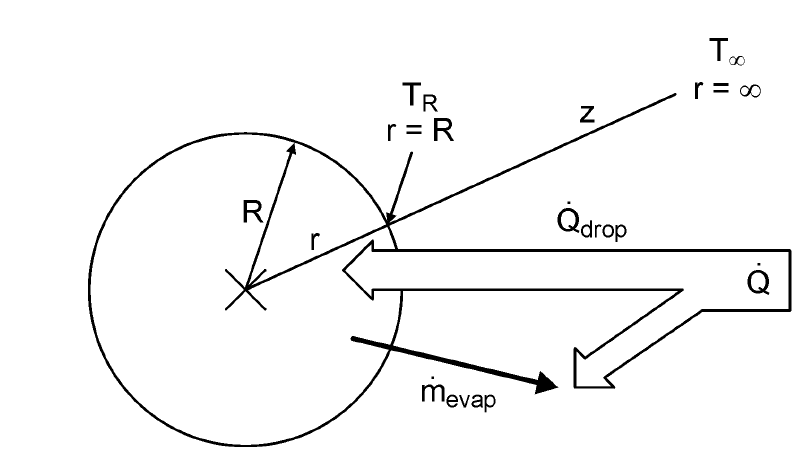
\includegraphics[width=\textwidth]{./imgs/spray_energy.png}
\end{block}  
 \end{column}
\end{columns}
%
\onslide<3->
\footnotesize
\begin{tabular}{|l|}
\hline \\
Correlação de Ranz \& Marshall:  $Nu= 2.0 +0.6 Re^{1/2} Pr^{1/3}$.\\ \\
\hline 
\end{tabular}
%
\end{frame}
%
\begin{frame}
\begin{block}{Transferência de Massa}
 \begin{itemize}
  \item<2-> Líquido e vapor em equilíbrio na superfície da gota.
  \begin{equation*}
  Y_{ac,s} = \frac{p_v \left(T_d\right)}{p_0}\frac{W_{ac}}{W} 
  \end{equation*}
  \item<3-> Equações da continuidade e das espécies para o vapor na vizinhança da gota:
\begin{equation*}
 \frac{dm_d}{dt} = -2\pi D \mathcal{D}_{ac} \rho_{ac} ln \left(
\frac{1-Y_{ac,\infty}}{1-Y_{ac,s}} \right) Sh 
\end{equation*}
 \end{itemize}
\end{block}

\onslide<4->
\vspace{10pt}
\footnotesize
\begin{tabular}{|l|}
\hline \\
Correlação de Ranz \& Marshall:  $ Sh = 2.0 +0.6 Re^{1/2} Sc^{1/3}$.\\ \\
\hline 
\end{tabular}
\end{frame}
%
\section{Cálculo Numérico}
\frame{\tableofcontents[currentsection]}
%
\begin{frame}[fragile] % Notice the [fragile] option %
\frametitle{Cálculo Numérico}
\begin{block}<2->{Método de Volumes Finitos}
\begin{itemize}
  \item<2-> Discretização da geometria;
  \item<2-> Discretização das equações;
  \item<2-> Algoritmo de solução do sistema de equações;
\end{itemize}
\end{block}

\onslide<3->
\begin{figure}\centering

\includegraphics[width=0.35\textwidth]{./imgs/foam_logo.png}\footnote<3->{http://www.openfoam.org}
\end{figure}

\end{frame}
%
\begin{frame}
\frametitle{Discretização do Espaço}
\begin{itemize}
  \item Malha ortogonal 2D (axissimétrica);
  \item Malha fina: $14.800$ células ($74 \times 200$);
  \item Malha grossa: $5.460$ células ($42 \times 130$);
\end{itemize}
\centering 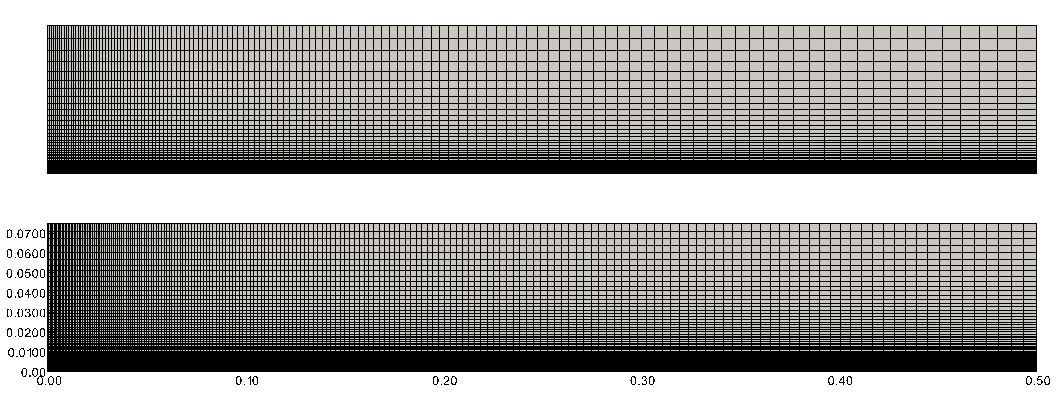
\includegraphics[width=\textwidth]{./imgs/grid.png}
\end{frame}
%
\begin{frame}
\frametitle{Discretização das Equações}
\begin{block}<1->{}
\begin{equation*}
 \underbrace{\frac{\partial \rho \phi}{\partial t}}_{\text{derivada temporal}} + \underbrace{\nabla \cdot \left(\rho \bv{U} \phi \right)}_{\text{advecção}} - \underbrace{\nabla \cdot \left( \rho \Gamma_{\phi} \nabla \phi \right)}_{\text{difusão}} = \underbrace{S\left(\phi\right)}_{\text{fontes}}
\end{equation*}
\end{block}
\begin{block}<2->{}
\begin{itemize}
  \item<2-> Tempo: Euler implícito;
  \item<3-> Advecção: teorema de Gauss + interpolação \textit{upwind};
  \item<4-> Difusão: teorema de Gauss + interpolação linear + diferença centrada;
  \item<5-> Fontes: tratamento explícito.
\end{itemize}
\end{block}
\end{frame}
%
\begin{frame}
\frametitle{O Algoritmo de Solução}
\begin{block}<1->{}
\begin{itemize}
  \item<2-> Sistemas lineares segregados;
  \item<3-> Acoplamento das variáveis: algoritmo PISO;
\end{itemize}
\end{block}
\end{frame}
%
\section{Resultados}
\frame{\tableofcontents[currentsection]}

\subsection{O Jato Turbulento}
\frametitle{Perfis Auto-Similares do Jato Turbulento (fase gasosa)}
\begin{frame}
\begin{overprint}
\onslide<1>
\begin{figure}
\centering
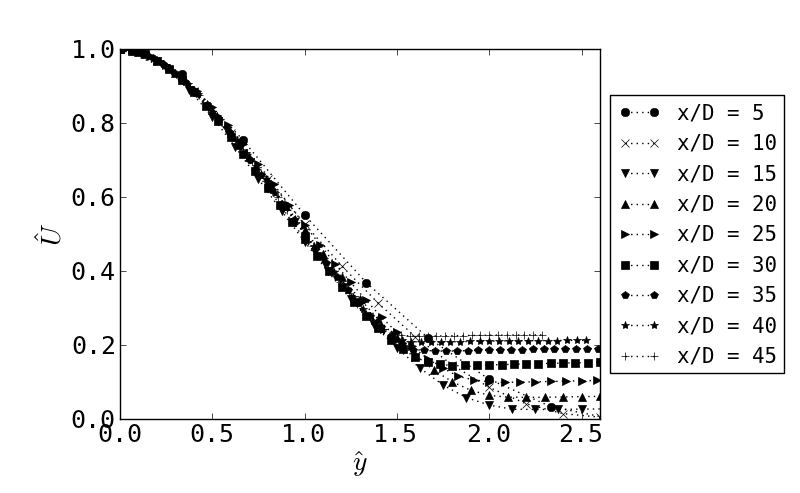
\includegraphics[width=0.85\textwidth]{../thesis/figuras/selfsimilar/selfsimilar_U.png}
\caption{Perfis auto-similares de velocidade adimensional ($\hat{U}$).}
\end{figure}

\onslide<2>
\begin{figure}
\centering
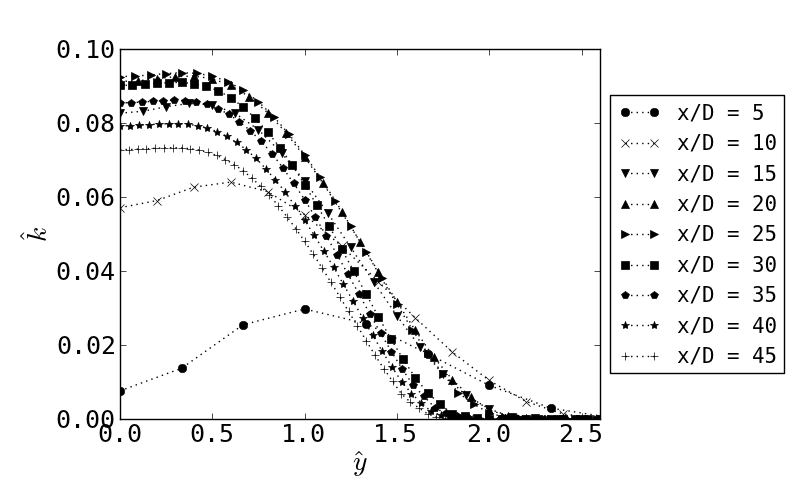
\includegraphics[width=0.85\textwidth]{../thesis/figuras/selfsimilar/selfsimilar_k.png}
\caption{Perfis auto-similares de energia cinética turbulenta adimensional ($\hat{k}$).}
\end{figure}

\onslide<3>
\begin{figure}
\centering
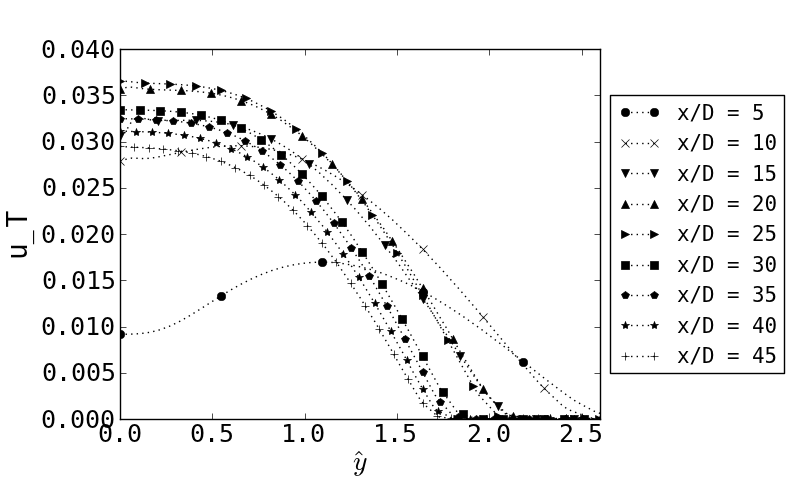
\includegraphics[width=0.85\textwidth]{../thesis/figuras/selfsimilar/selfsimilar_nut.png}
\caption{Perfis auto-similares da viscosidade turbulenta adimensional ($\hat{\nu}_T$). Superestimação: $\hat{\nu}_T=0.047 > \underbrace{0.029}_{\text{(POPE,2000)}}$.}
\end{figure}
\end{overprint}
\end{frame}
%
\begin{frame}
 \begin{figure}[!htb]
 \centering
\begin{tabular}{c}
 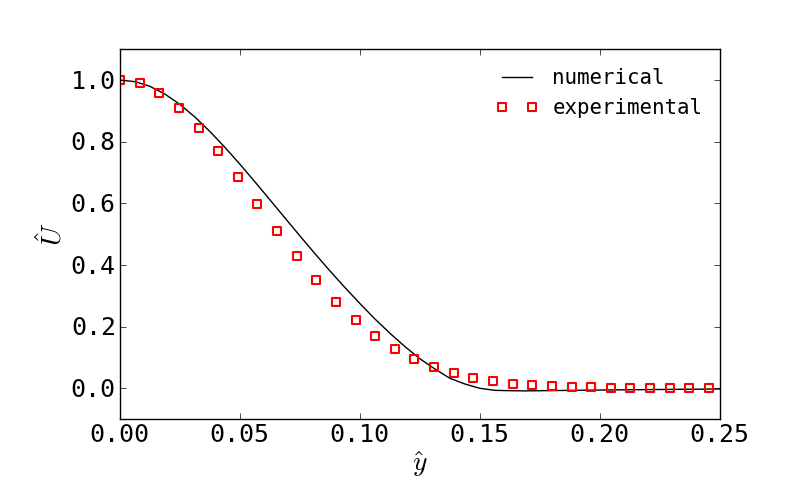
\includegraphics[width=0.85\textwidth]{../thesis/figuras/selfsimilar/selfsimilar_num_exp.png}
\end{tabular}
 \caption{Comparação do perfis numérico e experimental (Chen et al., 2006) de $\hat{U}$.}
\end{figure}
\end{frame}
%
\begin{frame}
 \begin{figure}[!htb]
 \centering
\begin{tabular}{c}
 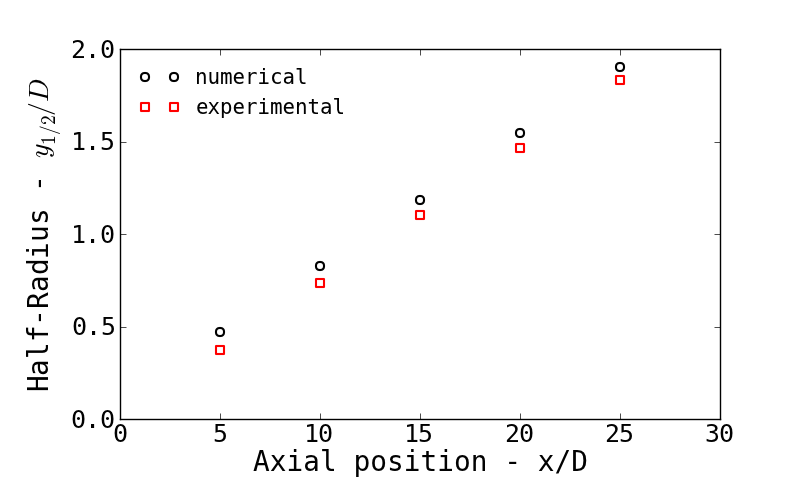
\includegraphics[width=0.75\textwidth]{../thesis/figuras/selfsimilar/selfsimilar_spread.png}
\end{tabular}
 \caption{Raio médio numérico e experimental (Chen et al., 2006).}
\end{figure}

%\vspace{5pt}
\footnotesize
\begin{tabular}{|l|}
\hline \\
$(d y_{1/2}/dx)_{\text{num}}$ $\sim 20\%$ maior do que $(d y_{1/2}/dx)_{\text{exp}}$.\\ \\
\hline 
\end{tabular}
\end{frame}
%
\subsection{Velocidade das Fases}
\begin{frame}[plain]{Velocidade Axial Média da Fase Gasosa ($\tilde{U}_x$)}
 \begin{figure}[!htb]
 \centering
\begin{tabular}{cc}
 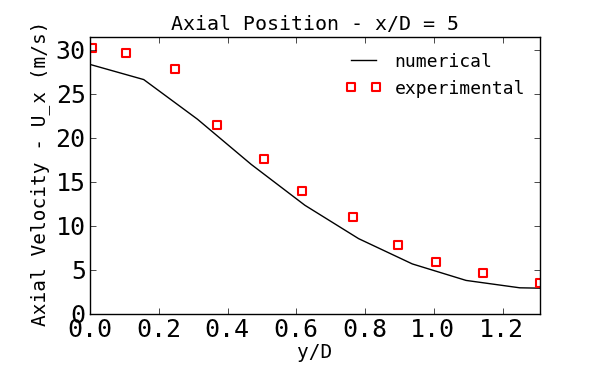
\includegraphics[width=0.45\textwidth]{../thesis/figuras/Ux/Ux_gas5.png} & 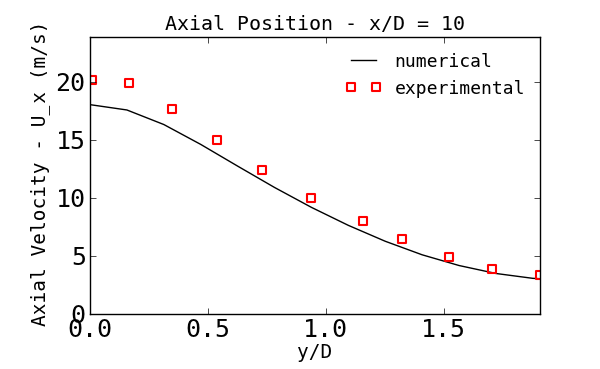
\includegraphics[width=0.45\textwidth]{../thesis/figuras//Ux/Ux_gas10.png} \\
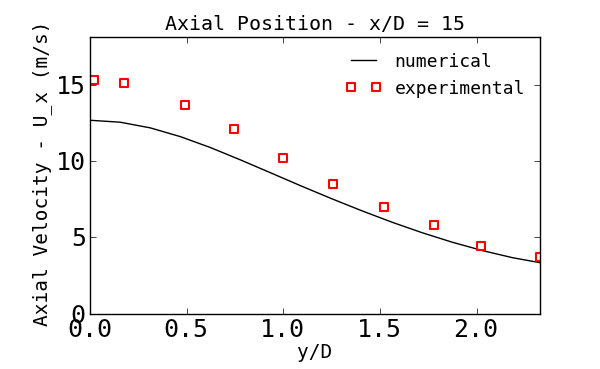
\includegraphics[width=0.45\textwidth]{../thesis/figuras/Ux/Ux_gas15.png} & 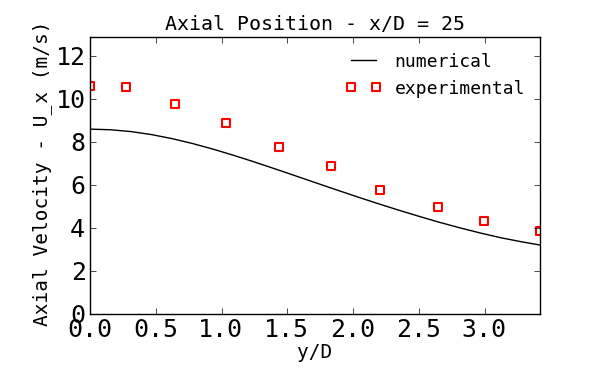
\includegraphics[width=0.45\textwidth]{../thesis/figuras/Ux/Ux_gas25.png}  
\end{tabular}
 \caption{Velocidade da fase gasosa. Numérico e experimental (Chen et al., 2006).}
 \label{fig: Ux_gas}
\end{figure}
\end{frame}


\begin{frame}[plain]{{Flutuação da Velocidade da Fase Gasosa ($< U''>$)}}
 \begin{figure}[!htb]
 \centering
\begin{tabular}{cc}
 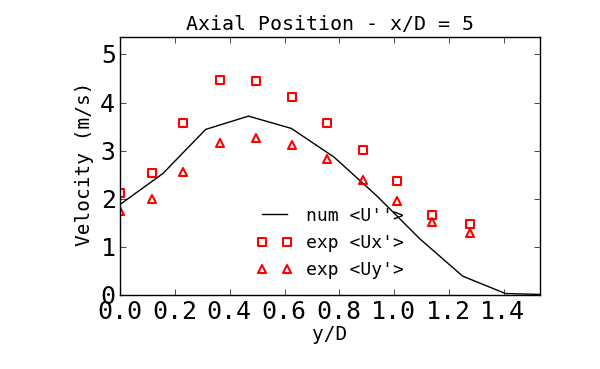
\includegraphics[width=0.5\textwidth]{../thesis/figuras/UU/UUx5.png} & 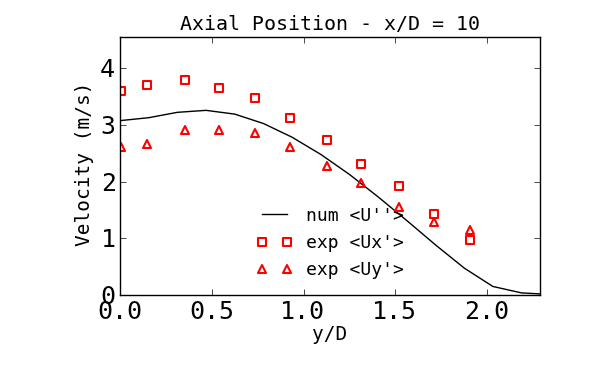
\includegraphics[width=0.5\textwidth]{../thesis/figuras/UU/UUx10.png} \\
  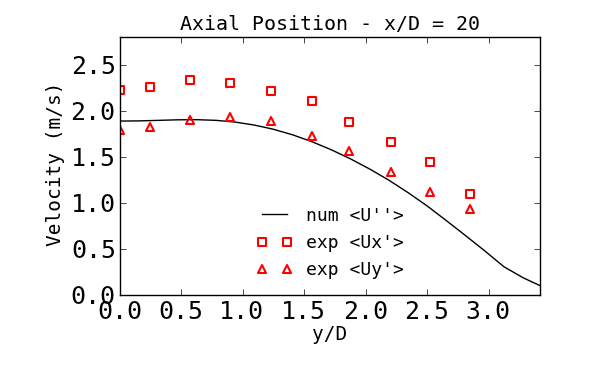
\includegraphics[width=0.5\textwidth]{../thesis/figuras//UU/UUx20.png} & 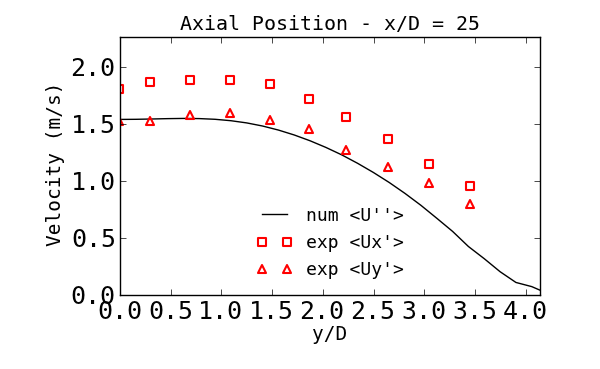
\includegraphics[width=0.5\textwidth]{../thesis/figuras/UU/UUx25.png}
\end{tabular}
 \caption{\footnotesize Numérico $<U''>$ e experimental $<U''_x>$ e $<U''_y>$ (Chen et al., 2006).}
\end{figure}
\end{frame}

\begin{frame}[plain]{Velocidade das Gotas}
 \begin{figure}[!htb]
 \centering
\begin{tabular}{cc}
 \includegraphics[width=0.45\textwidth]{../thesis/figuras/Ux/Ux5.png} & \includegraphics[width=0.45\textwidth]{../thesis/figuras//Ux/Ux10.png} \\
\includegraphics[width=0.45\textwidth]{../thesis/figuras//Ux/Ux20.png} & \includegraphics[width=0.45\textwidth]{../thesis/figuras/Ux/Ux25.png}
\end{tabular}
 \caption{ \footnotesize Velocidade das gotas da classe ($D \in [10,20] \mu m$). Numérico e experimental (Chen et al., 2006).}
\end{figure}
\end{frame}



% \begin{frame}
% \begin{figure}[!htb]
%  \centering
% \begin{tabular}{cc}
%  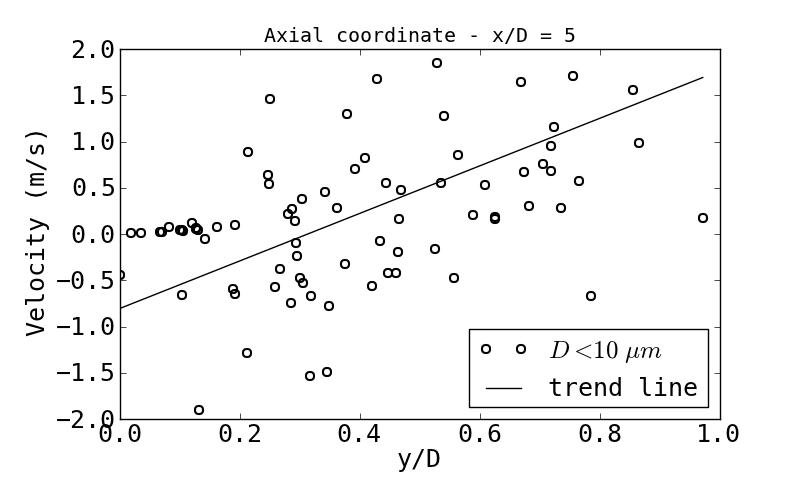
\includegraphics[width=0.5\textwidth]{../thesis/figuras/dispersion/class0_5.png} & 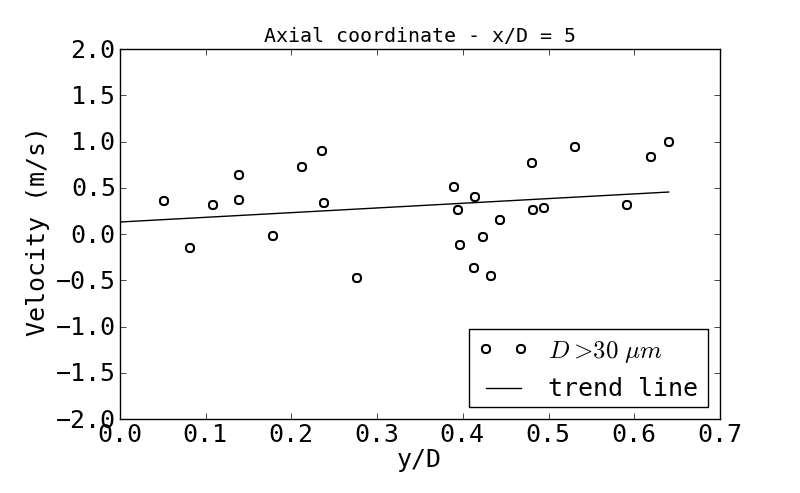
\includegraphics[width=0.5\textwidth]{../thesis/figuras/dispersion/class4_5.png} \\
%  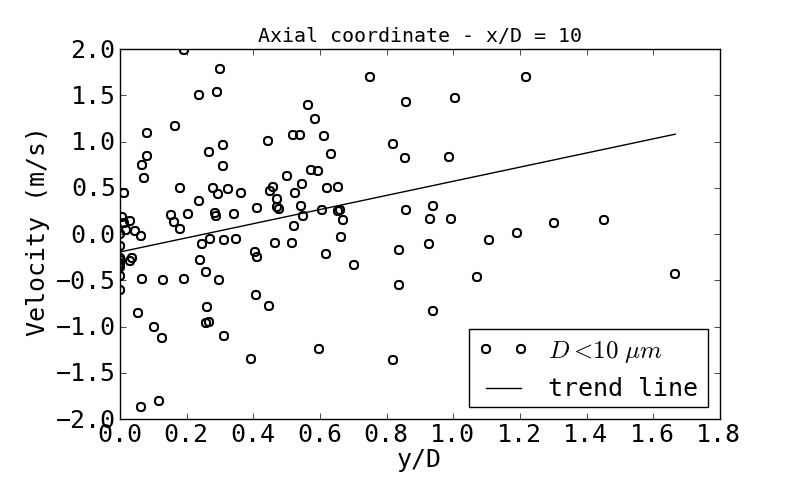
\includegraphics[width=0.5\textwidth]{../thesis/figuras/dispersion/class0_10.png} & 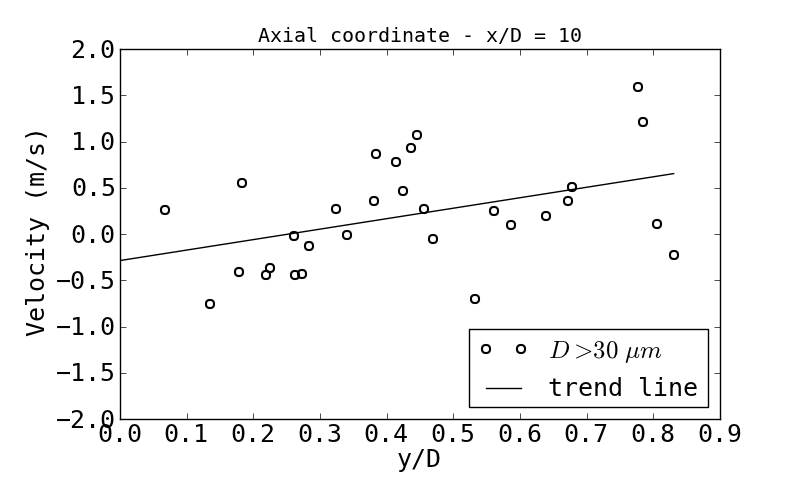
\includegraphics[width=0.5\textwidth]{../thesis/figuras/dispersion/class4_10.png} \\
%  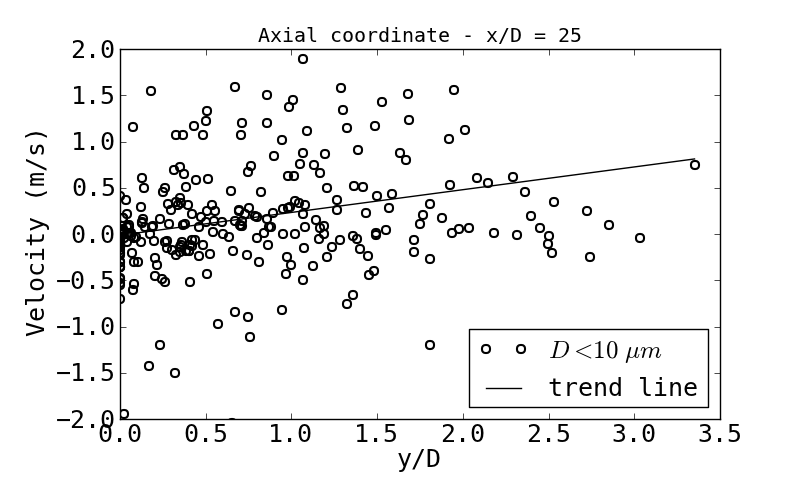
\includegraphics[width=0.5\textwidth]{../thesis/figuras/dispersion/class0_25.png} & 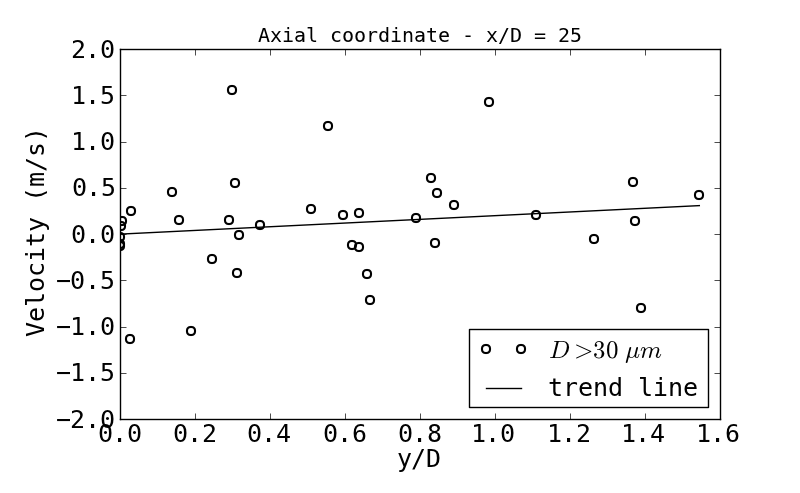
\includegraphics[width=0.5\textwidth]{../thesis/figuras/dispersion/class4_25.png} \\
% \end{tabular}
%  \caption{Scatter plot of the numerical radial fluctuating velocity of droplets ($U''_{y}$) in two different size classes: $D< 10\ \mu m$ on the left or (a), (c) and (e) labels; and $D> 30\ \mu m$ on the right or (b), (d) and (f) labels. The dispersion in the radial velocity is higher for the smaller droplet class and in the vicinity of the nozzle exit.}
% \label{fig: jointUV}
% \end{figure}
% \end{frame}

\subsection{Vazão Mássica das Gotas e do Vapor}
\begin{frame}{Vazão Mássica de Líquido}
\begin{figure}[!htb]
\centering
  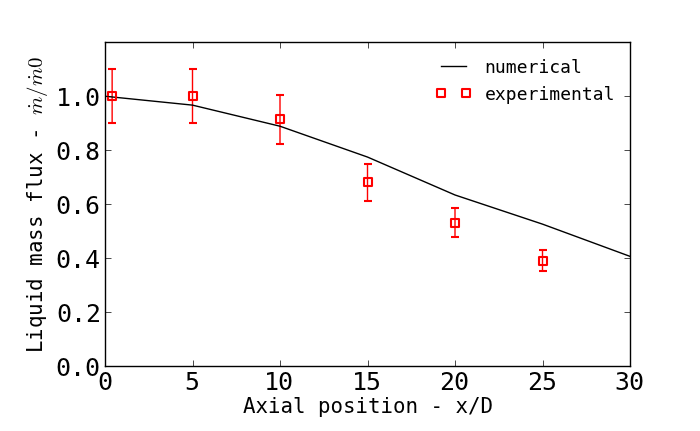
\includegraphics[width=0.8\textwidth]{../thesis/figuras/drop_mflux.png}
\caption{Vazão de massa na fase líquida. Numérico e experimental (Chen et al., 2006).}
\label{fig: droplet_flux}
\end{figure} 
\end{frame}

\begin{frame}[plain]{Fluxo Mássico de Vapor}  % notice the fragile option, since the body
\begin{figure}[!htb]
 \centering
\begin{tabular}{ccc}
 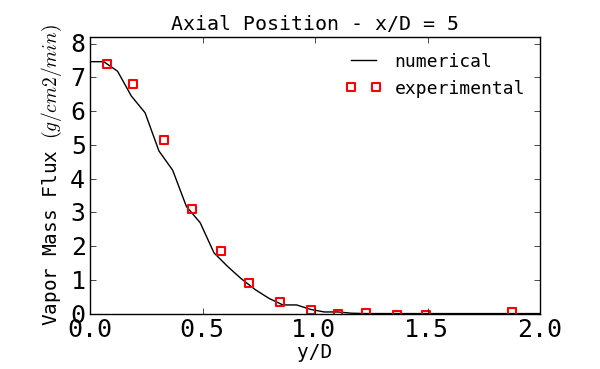
\includegraphics[width=0.45\textwidth]{../thesis/figuras/mvapor/mvapor5.png} & 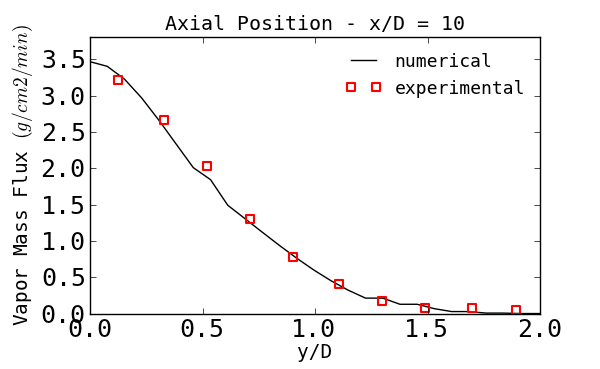
\includegraphics[width=0.45\textwidth]{../thesis/figuras/mvapor/mvapor10.png} \\
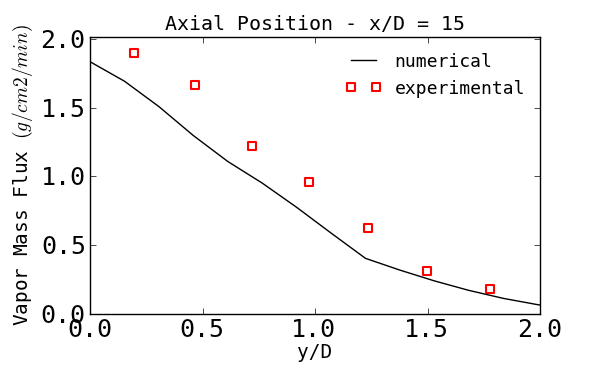
\includegraphics[width=0.45\textwidth]{../thesis/figuras/mvapor/mvapor15.png} & 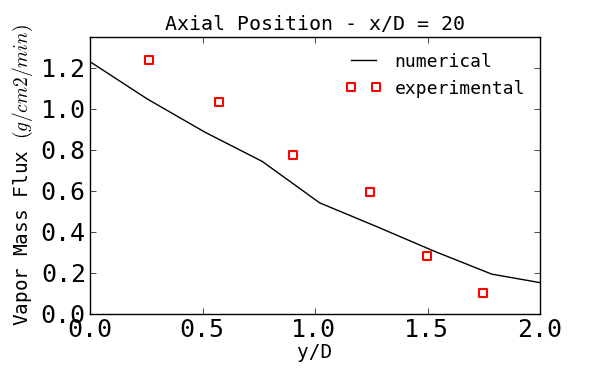
\includegraphics[width=0.45\textwidth]{../thesis/figuras//mvapor/mvapor20.png}
\end{tabular}
 \caption{\footnotesize Fluxo mássico de vapor: $\dot{m}''_{ac}=\rho \bar{Y}_{ac} \tilde{U}_x$. Numérico e experimental (Chen et al., 2006).}
\end{figure}
\end{frame}

\begin{frame}[plain]{Diâmetro de Sauter}  % notice the fragile option, since the body
\begin{figure}[!htb]
 \centering
\begin{tabular}{cc}
 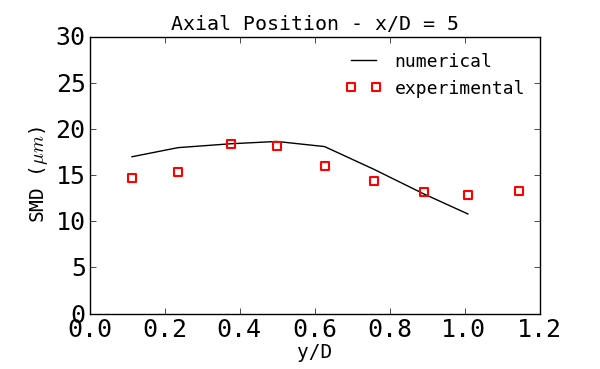
\includegraphics[width=0.5\textwidth]{../thesis/figuras/smd/smd5.png} &
 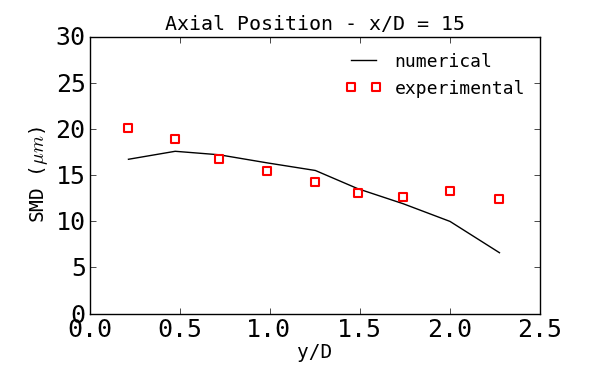
\includegraphics[width=0.5\textwidth]{../thesis/figuras/smd/smd15.png} \\
 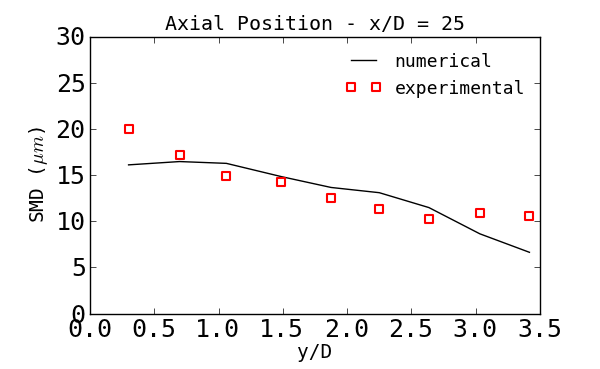
\includegraphics[width=0.5\textwidth]{../thesis/figuras/smd/smd25.png} \\
\end{tabular}
 \caption{\footnotesize Diâmetro de Sauter (SMD). Numérico e experimental (Chen et al., 2006).}
\end{figure}
\end{frame}
%
\begin{frame}[plain]
\frametitle{Temperatura da Fase Gasosa}
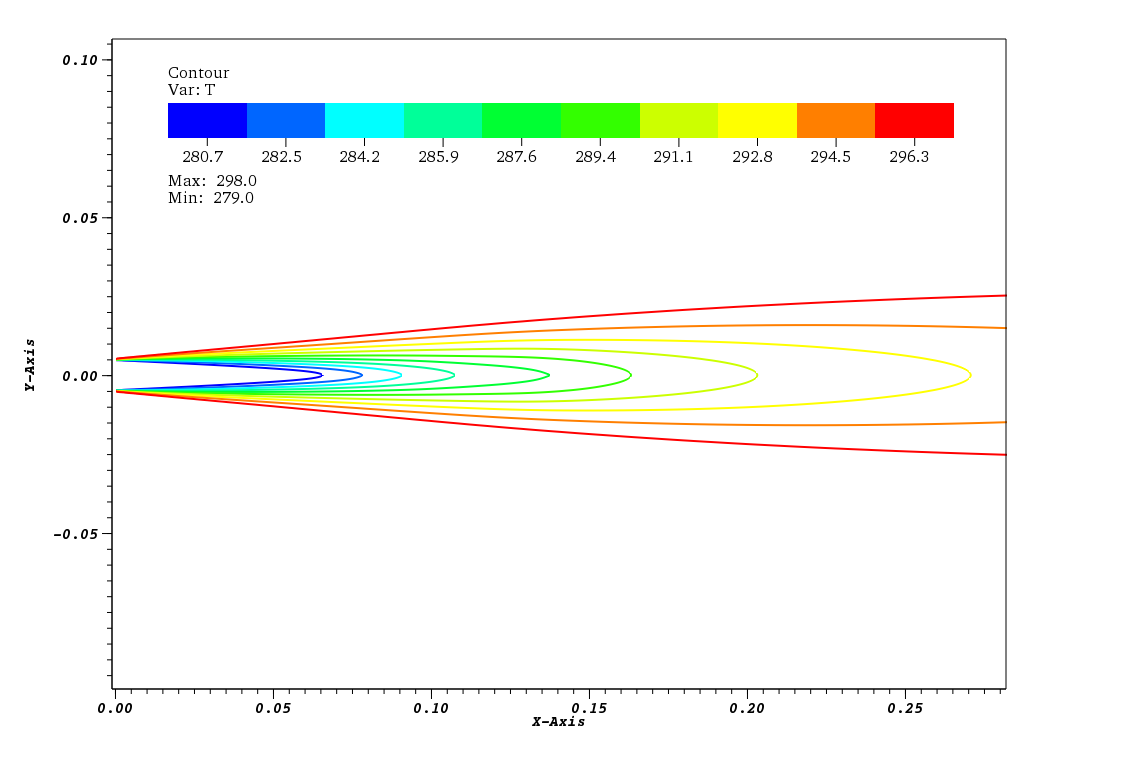
\includegraphics[width=\textwidth]{./imgs/visit/T.png}
\end{frame}
%
\begin{frame}[plain]
\frametitle{Densidade da Fase Gasosa}
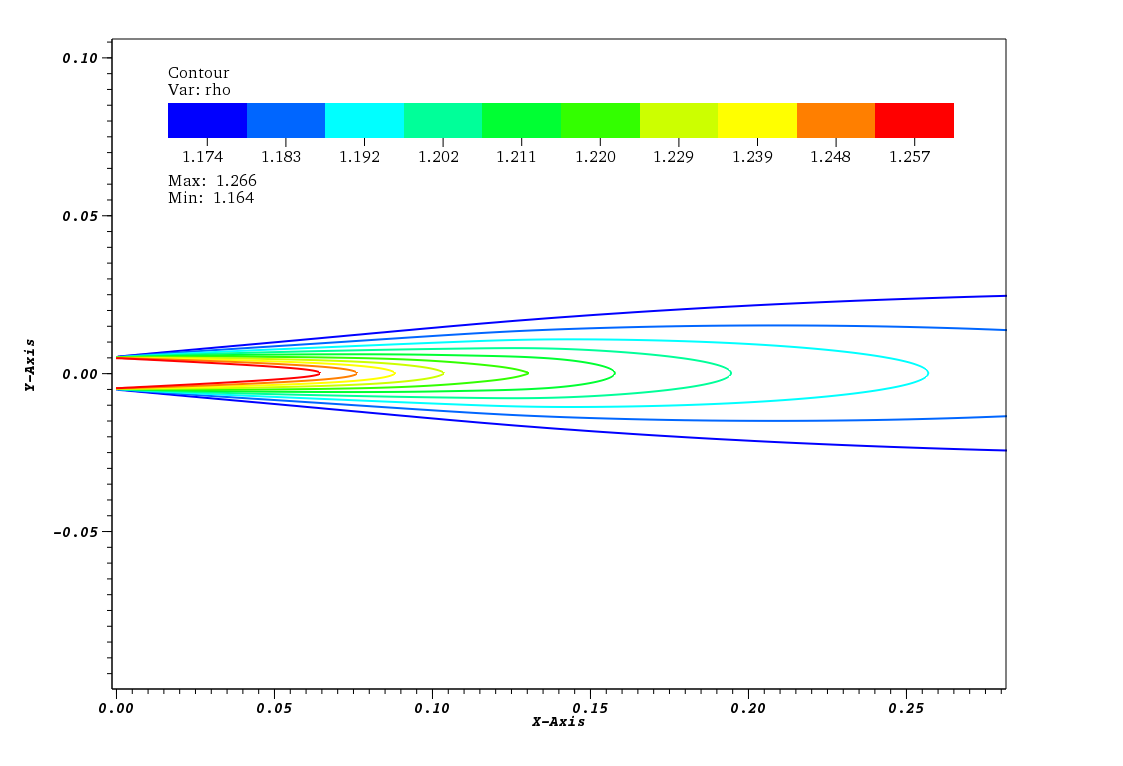
\includegraphics[width=\textwidth]{./imgs/visit/rho.png}
\end{frame}
%
\begin{frame}[plain]
\frametitle{Energia Cinética Turbulenta}
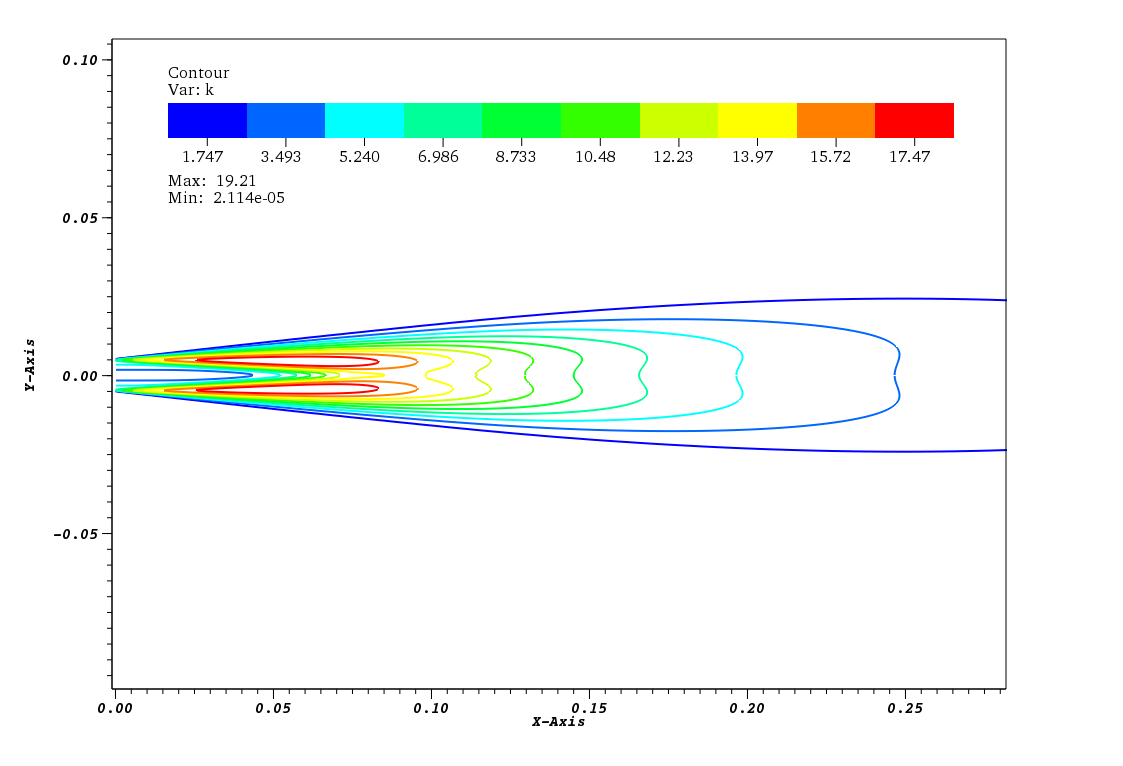
\includegraphics[width=\textwidth]{./imgs/visit/k.png}
\end{frame}
%
\begin{frame}[plain]
\frametitle{Viscosidade Turbulenta}
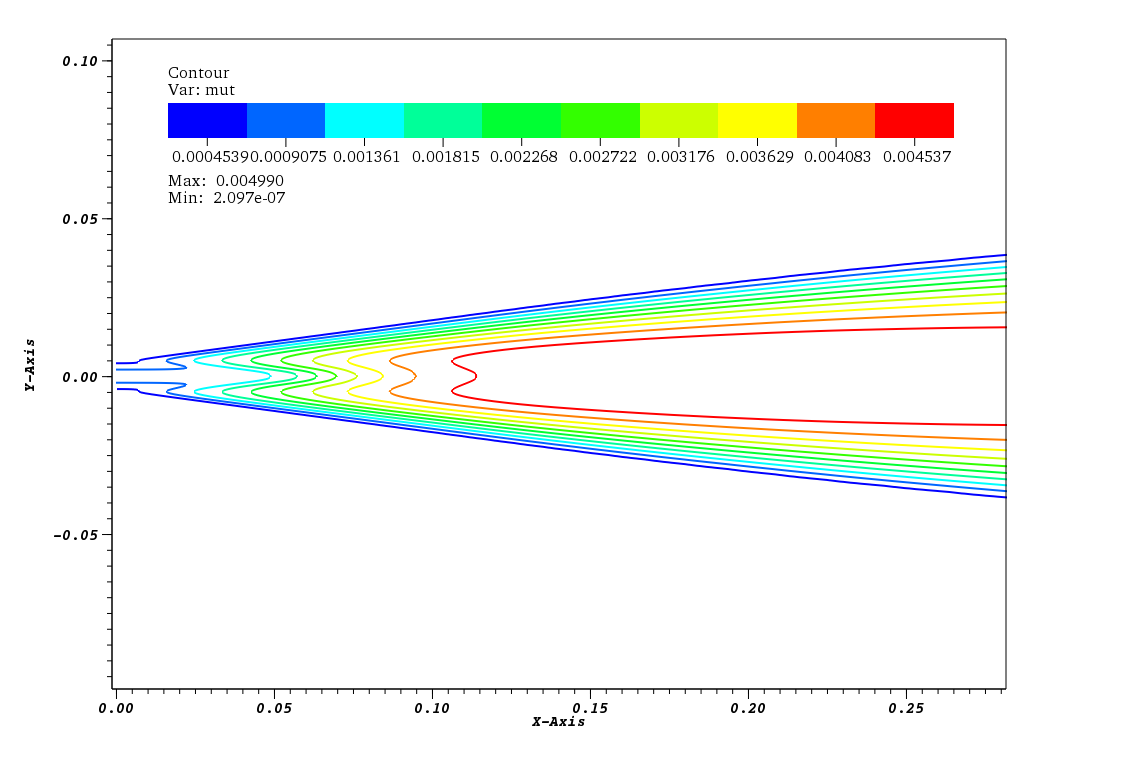
\includegraphics[width=\textwidth]{./imgs/visit/mut.png}
\end{frame}
%
\begin{frame}[plain]
\frametitle{Velocidade das Gotas}
\begin{center}
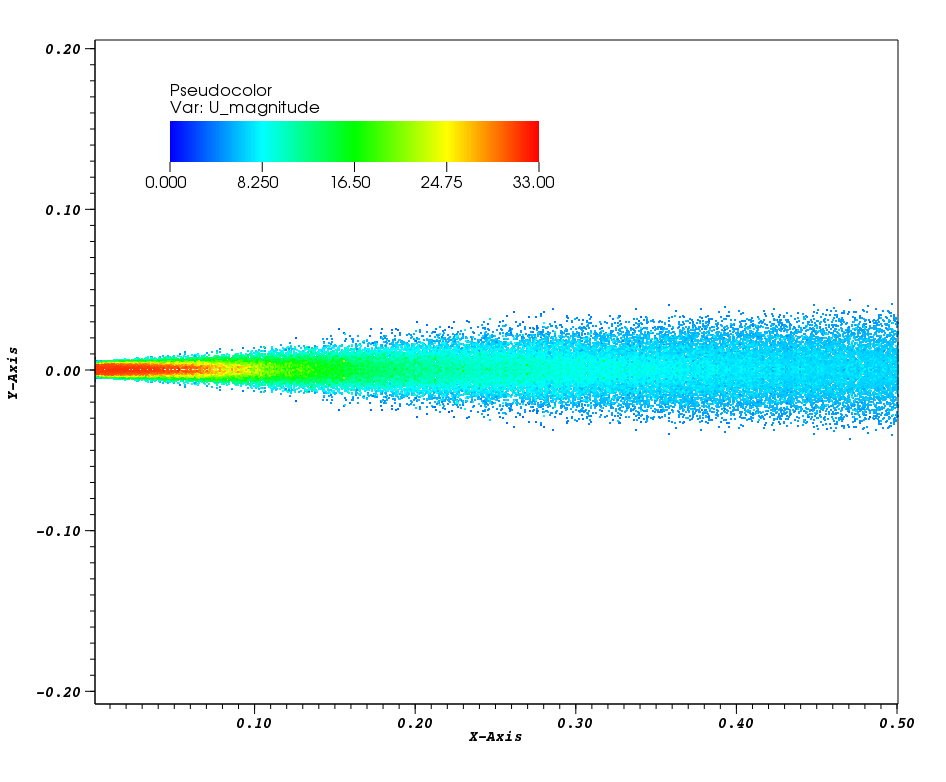
\includegraphics[height=\textheight]{./imgs/visit/drop_U.png}
\end{center}
\end{frame}
%
\begin{frame}[plain]
\frametitle{Temperatura das Gotas}
\begin{center}
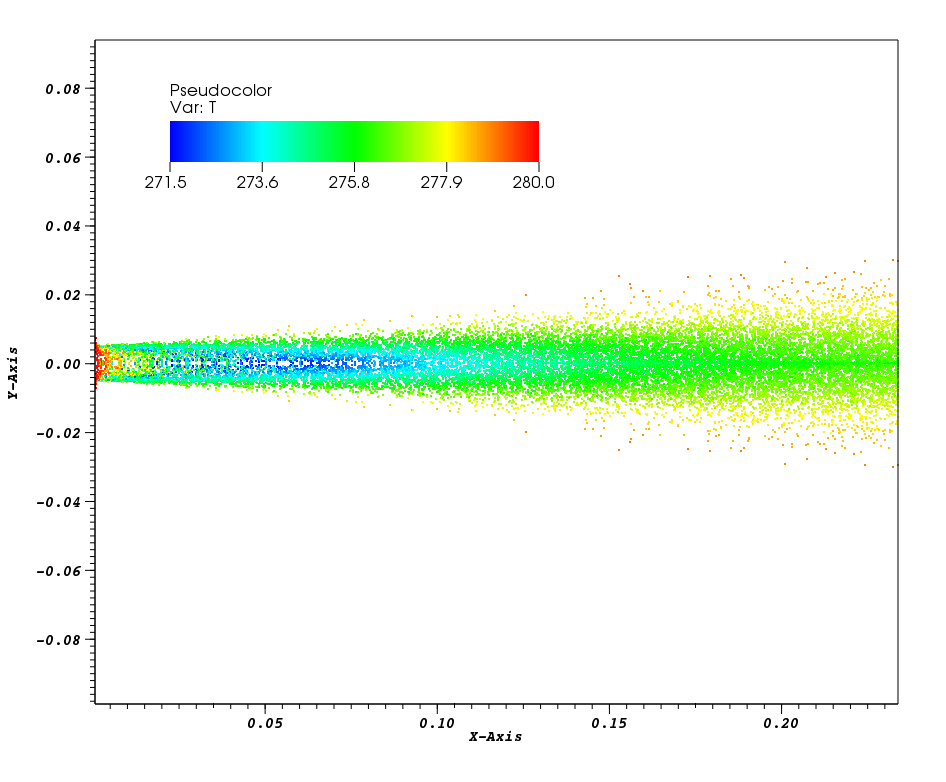
\includegraphics[height=\textheight]{./imgs/visit/drop_T.png}
\end{center}
\end{frame}
%

\section{Conclusões}
\frame{\frametitle{Resumo} \tableofcontents}
\frame{\tableofcontents[currentsection]}

\begin{frame}

\begin{block}{Formulação}
  \begin{itemize}
  \item $M \rightarrow  0 \Longrightarrow$  métodos numéricos para escoamento incompressível;
  \item O método Euleriano-Lagrangiano é uma \textit{boa} descrição computacional para a fase dispersa.
 \end{itemize}
\end{block}


\begin{block}{Numérico $\times$ Experimental:}
 \begin{itemize}
  \item $\bv{\tilde{U}}$, $\bv{U}_d$ e $\dot{m}_d$ \textbf{sub}estimados;
  \item $\text{k-epsilon} \Longrightarrow \mu_T$ \textbf{super}estimado.
 \end{itemize}
\end{block}

\begin{block}{Trabalhos Futuros:}
 \begin{itemize}
  \item $\dot{h}_{d}$, $\dot{m}_d \Longleftarrow \text{turbulência}$;
  \item $Sc,\ Pr \neq 1$;
  \item Tratar termos fontes de forma \textit{mais implícita}.
 \end{itemize}
\end{block}
\end{frame}


\begin{frame}
\centerline{Obrigado pela atenção.}
\end{frame}
% End of slides
\end{document} 
